\section{O Mestre das Chaves: Cofre Bitwarden \faKey}

O nome do seu cachorro não é uma senha segura, e anotar senhas em um caderno é muito perigoso. O segredo da segurança não é a dificuldade (símbolos estranhos), é o \textbf{TAMANHO}. 

\vspace{0.3cm}
Tentar decorar senhas para 50 sites diferentes é impossível. É por isso que usamos um \textbf{Gerenciador de Senhas}.

\vspace{0.3cm}
\begin{figure}[h]
	\centering
	%\imagemSuave[0.6\textwidth]{imagens/cofre_bitwarden.png} 
	
\includegraphics[width=0.6\textwidth]{imagens/bitwarden_logo.png}
		\caption*{(\citeauthor{bitwarden_app} \citefield{bitwarden_app}{version} - Versão oficial)}
\end{figure}

\subsection*{Como criar o seu Cofre Digital:}
\begin{enumerate}
	\item Baixe o aplicativo \textbf{Bitwarden} no seu celular.

	\begin{center}
		\begin{minipage}{\linewidth}
			
			\begin{minipage}{0.3\linewidth}
				\centering
				\textbf{\textcolor{BraveOrange}{\faAndroid \ Android}}\\[0.2cm]
				\href{https://bfaxke.short.gy/bitwarden-android}{
					
\includegraphics[width=0.8\linewidth]{imagens/qr_bitwarden_android.png}
				}\\[0.1cm]
				{\scriptsize (Toque ou escaneie)}
			\end{minipage}
			\hfill
			\begin{minipage}{0.3\linewidth}
				\centering
				\textbf{\textcolor{NordText}{\faApple \ iOS / iPhone}}\\[0.2cm]
				\href{https://bfaxke.short.gy/bitwarden-apple}{
					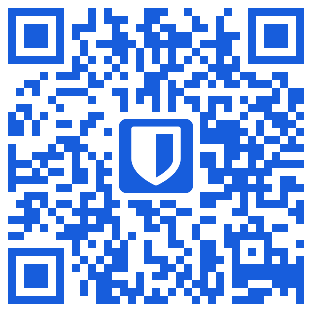
\includegraphics[width=0.8\linewidth]{imagens/qr_bitwarden_ios.png}
				}\\[0.1cm]
				{\scriptsize (Toque ou escaneie)}
			\end{minipage}
			\hfill
			\begin{minipage}{0.3\linewidth}
				\centering
				\textbf{\textcolor{BitwardenBlue}{\faDesktop \ Computador}}\\[0.2cm]
				\href{https://bfaxke.short.gy/bitwarden-desktop}{
					
\includegraphics[width=0.8\linewidth]{imagens/qr_bitwarden_desktop.png}
				}\\[0.1cm]
				{\scriptsize (Para Windows/Linux/Mac)}
			\end{minipage}
			
		\end{minipage}
	\end{center}
	
	\item Crie uma conta usando o seu e-mail.
	\item Invente UMA única \textbf{\enquote{Senha Mestra}}. Use uma frase longa que faça sentido para você (Exemplo: \textit{\enquote{Eu amo bolo de cenoura com cafe}}).
	\item Vá nas \textit{Configurações > Segurança} do aplicativo e ative o \textbf{Desbloqueio por Biometria} (Impressão Digital).
\end{enumerate}

\subsection*{Passo a Passo para Configurar o Bitwarden:}

\subsection*{Muito Além das Senhas: Sua Carteira Blindada}

O Bitwarden não guarda apenas senhas. Ele é um cofre digital completo desenhado para substituir a sua carteira física e a sua agenda de anotações. Ao clicar no botão de adicionar (\textbf{+}), você descobrirá diferentes \enquote{Tipos} de documentos que podem ser trancados com a sua biometria:

\begin{itemize}
	\item \textbf{Cartões de Crédito:} Guarde os dados dos seus cartões físicos e virtuais de forma criptografada. É infinitamente mais seguro do que deixar salvo no bloco de notas do celular ou tirar foto do cartão.
	\item \textbf{Identidades:} Salve seu CPF, RG, Passaporte e Endereço completo. Assim, quando for preencher um formulário longo em um site seguro, o Bitwarden preenche tudo para você.
	\item \textbf{Anotações Seguras:} Sabe a senha do Roteador Wi-Fi ou aquele \enquote{Código de Recuperação} do WhatsApp? Crie uma anotação segura para que só você tenha acesso.
\end{itemize}

\subsection*{A Configuração do PIN e a Pergunta Crítica}

Ao configurar o acesso rápido (Biometria ou PIN) para não ter que digitar sua frase-senha o tempo todo, o aplicativo fará uma pergunta muito importante: \textbf{\enquote{Exigir senha principal no reinício do aplicativo?}}

\begin{figure}[h]
	\centering
	% Substitua pelo nome do seu arquivo da Imagem 6
	\imagemSuave[0.6\linewidth]{imagens/bitwarden_aviso_reinicio.png}
\end{figure}

\begin{tcolorbox}[colback=NordBackground, colframe=BraveOrange, coltext=white, title=\faShieldAlt \ Qual a diferença entre Sim e Não?]
	\textbf{Se você escolher \enquote{NÃO}:} O aplicativo deixará uma cópia da sua chave do cofre no celular, protegida apenas pelo seu PIN. É prático, mas se o seu celular for roubado, um PIN de 4 números é fácil de ser quebrado por criminosos.
	
	\textbf{Se você escolher \enquote{SIM} (Nossa Recomendação):} O celular nunca guarda a chave. Se o aparelho for roubado e desligado, o cofre se tranca totalmente. Quando o celular for reiniciado, você terá que digitar a sua \enquote{Senha Mestra} (a frase longa) uma vez para reabrir o cofre. No dia a dia normal, o seu PIN e a sua digital continuarão funcionando rapidamente!
\end{tcolorbox}

\begin{tcolorbox}[colback=NordBackground, colframe=BraveOrange, title=\faExclamationTriangle\ A Regra de Ouro]
	\textcolor{white}{O Bitwarden não possui a opção \enquote{Esqueci minha senha}. Anote a sua Senha Mestra em um pedaço de papel e guarde no fundo de uma gaveta segura na sua casa. Se esquecer a senha mestra, o cofre ficará trancado para sempre!}
\end{tcolorbox}